\section{Definition}

We already explained the idea of the problem in the introduction, hereunder we
formally define Sorting Under Partial Information.

Quoting from \cite{cardinal2013sorting},

\begin{quotation}
Let $V = \enum{v_1 , \cdots , v_n}$ be a set
equipped with an unknown linear order. Given a subset of the relations $v_i
\leq v_j$, determine the complete linear order by queries of the form: ``is
$v_i \leq v_j$ ?''.
\end{quotation}


\begin{figure} \centering 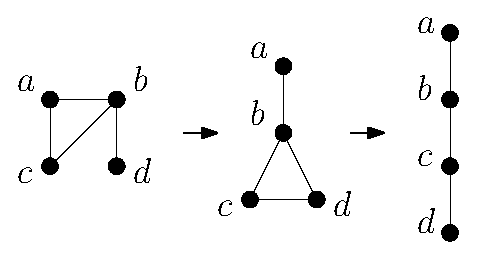
\includegraphics[height=0.2\textheight]{fig/supi/ex2}
\caption{An instance of the problem of sorting under partial information. In
this example, we use 2 comparisons (dashed edges). At every step, the Hasse
diagram of the currently known partial order is shown.}
\label{fig:supi:def:ex2} \end{figure}


\ref{fig:supi:def:ex2} shows an example of an instance of Sorting Under Partial
Information. Note that in this example we only ask the minimal number of
questions needed to solve the problem. We could have asked $a \ask{\le}
d$ as the first question but then we would have still had to ask 2 more
questions.
